% Options for packages loaded elsewhere
\PassOptionsToPackage{unicode}{hyperref}
\PassOptionsToPackage{hyphens}{url}
%
\documentclass[
]{article}
\usepackage{amsmath,amssymb}
\usepackage{lmodern}
\usepackage{ifxetex,ifluatex}
\ifnum 0\ifxetex 1\fi\ifluatex 1\fi=0 % if pdftex
  \usepackage[T1]{fontenc}
  \usepackage[utf8]{inputenc}
  \usepackage{textcomp} % provide euro and other symbols
\else % if luatex or xetex
  \usepackage{unicode-math}
  \defaultfontfeatures{Scale=MatchLowercase}
  \defaultfontfeatures[\rmfamily]{Ligatures=TeX,Scale=1}
\fi
% Use upquote if available, for straight quotes in verbatim environments
\IfFileExists{upquote.sty}{\usepackage{upquote}}{}
\IfFileExists{microtype.sty}{% use microtype if available
  \usepackage[]{microtype}
  \UseMicrotypeSet[protrusion]{basicmath} % disable protrusion for tt fonts
}{}
\makeatletter
\@ifundefined{KOMAClassName}{% if non-KOMA class
  \IfFileExists{parskip.sty}{%
    \usepackage{parskip}
  }{% else
    \setlength{\parindent}{0pt}
    \setlength{\parskip}{6pt plus 2pt minus 1pt}}
}{% if KOMA class
  \KOMAoptions{parskip=half}}
\makeatother
\usepackage{xcolor}
\IfFileExists{xurl.sty}{\usepackage{xurl}}{} % add URL line breaks if available
\IfFileExists{bookmark.sty}{\usepackage{bookmark}}{\usepackage{hyperref}}
\hypersetup{
  pdftitle={ASSIGNMENT1..},
  pdfauthor={MUNERAH},
  hidelinks,
  pdfcreator={LaTeX via pandoc}}
\urlstyle{same} % disable monospaced font for URLs
\usepackage[margin=1in]{geometry}
\usepackage{color}
\usepackage{fancyvrb}
\newcommand{\VerbBar}{|}
\newcommand{\VERB}{\Verb[commandchars=\\\{\}]}
\DefineVerbatimEnvironment{Highlighting}{Verbatim}{commandchars=\\\{\}}
% Add ',fontsize=\small' for more characters per line
\usepackage{framed}
\definecolor{shadecolor}{RGB}{248,248,248}
\newenvironment{Shaded}{\begin{snugshade}}{\end{snugshade}}
\newcommand{\AlertTok}[1]{\textcolor[rgb]{0.94,0.16,0.16}{#1}}
\newcommand{\AnnotationTok}[1]{\textcolor[rgb]{0.56,0.35,0.01}{\textbf{\textit{#1}}}}
\newcommand{\AttributeTok}[1]{\textcolor[rgb]{0.77,0.63,0.00}{#1}}
\newcommand{\BaseNTok}[1]{\textcolor[rgb]{0.00,0.00,0.81}{#1}}
\newcommand{\BuiltInTok}[1]{#1}
\newcommand{\CharTok}[1]{\textcolor[rgb]{0.31,0.60,0.02}{#1}}
\newcommand{\CommentTok}[1]{\textcolor[rgb]{0.56,0.35,0.01}{\textit{#1}}}
\newcommand{\CommentVarTok}[1]{\textcolor[rgb]{0.56,0.35,0.01}{\textbf{\textit{#1}}}}
\newcommand{\ConstantTok}[1]{\textcolor[rgb]{0.00,0.00,0.00}{#1}}
\newcommand{\ControlFlowTok}[1]{\textcolor[rgb]{0.13,0.29,0.53}{\textbf{#1}}}
\newcommand{\DataTypeTok}[1]{\textcolor[rgb]{0.13,0.29,0.53}{#1}}
\newcommand{\DecValTok}[1]{\textcolor[rgb]{0.00,0.00,0.81}{#1}}
\newcommand{\DocumentationTok}[1]{\textcolor[rgb]{0.56,0.35,0.01}{\textbf{\textit{#1}}}}
\newcommand{\ErrorTok}[1]{\textcolor[rgb]{0.64,0.00,0.00}{\textbf{#1}}}
\newcommand{\ExtensionTok}[1]{#1}
\newcommand{\FloatTok}[1]{\textcolor[rgb]{0.00,0.00,0.81}{#1}}
\newcommand{\FunctionTok}[1]{\textcolor[rgb]{0.00,0.00,0.00}{#1}}
\newcommand{\ImportTok}[1]{#1}
\newcommand{\InformationTok}[1]{\textcolor[rgb]{0.56,0.35,0.01}{\textbf{\textit{#1}}}}
\newcommand{\KeywordTok}[1]{\textcolor[rgb]{0.13,0.29,0.53}{\textbf{#1}}}
\newcommand{\NormalTok}[1]{#1}
\newcommand{\OperatorTok}[1]{\textcolor[rgb]{0.81,0.36,0.00}{\textbf{#1}}}
\newcommand{\OtherTok}[1]{\textcolor[rgb]{0.56,0.35,0.01}{#1}}
\newcommand{\PreprocessorTok}[1]{\textcolor[rgb]{0.56,0.35,0.01}{\textit{#1}}}
\newcommand{\RegionMarkerTok}[1]{#1}
\newcommand{\SpecialCharTok}[1]{\textcolor[rgb]{0.00,0.00,0.00}{#1}}
\newcommand{\SpecialStringTok}[1]{\textcolor[rgb]{0.31,0.60,0.02}{#1}}
\newcommand{\StringTok}[1]{\textcolor[rgb]{0.31,0.60,0.02}{#1}}
\newcommand{\VariableTok}[1]{\textcolor[rgb]{0.00,0.00,0.00}{#1}}
\newcommand{\VerbatimStringTok}[1]{\textcolor[rgb]{0.31,0.60,0.02}{#1}}
\newcommand{\WarningTok}[1]{\textcolor[rgb]{0.56,0.35,0.01}{\textbf{\textit{#1}}}}
\usepackage{graphicx}
\makeatletter
\def\maxwidth{\ifdim\Gin@nat@width>\linewidth\linewidth\else\Gin@nat@width\fi}
\def\maxheight{\ifdim\Gin@nat@height>\textheight\textheight\else\Gin@nat@height\fi}
\makeatother
% Scale images if necessary, so that they will not overflow the page
% margins by default, and it is still possible to overwrite the defaults
% using explicit options in \includegraphics[width, height, ...]{}
\setkeys{Gin}{width=\maxwidth,height=\maxheight,keepaspectratio}
% Set default figure placement to htbp
\makeatletter
\def\fps@figure{htbp}
\makeatother
\setlength{\emergencystretch}{3em} % prevent overfull lines
\providecommand{\tightlist}{%
  \setlength{\itemsep}{0pt}\setlength{\parskip}{0pt}}
\setcounter{secnumdepth}{-\maxdimen} % remove section numbering
\ifluatex
  \usepackage{selnolig}  % disable illegal ligatures
\fi

\title{ASSIGNMENT1..}
\author{MUNERAH}
\date{9/24/2021}

\begin{document}
\maketitle

\begin{Shaded}
\begin{Highlighting}[]
\DocumentationTok{\#\#\# import the dataset into R }
\NormalTok{dataset }\OtherTok{\textless{}{-}}\FunctionTok{read.csv}\NormalTok{(}\StringTok{"C:/Users/mnooo/Desktop/Datasets/Student.csv"}\NormalTok{)}
\DocumentationTok{\#\# summary }
\FunctionTok{summary}\NormalTok{(dataset)}
\end{Highlighting}
\end{Shaded}

\begin{verbatim}
##        X         race.ethnicity     parental.level.of.education
##  Min.   :  0.0   Length:1000        Length:1000                
##  1st Qu.:249.8   Class :character   Class :character           
##  Median :499.5   Mode  :character   Mode  :character           
##  Mean   :499.5                                                 
##  3rd Qu.:749.2                                                 
##  Max.   :999.0                                                 
##     lunch           test.preparation.course math.percentage 
##  Length:1000        Length:1000             Min.   :0.0000  
##  Class :character   Class :character        1st Qu.:0.5700  
##  Mode  :character   Mode  :character        Median :0.6600  
##                                             Mean   :0.6609  
##                                             3rd Qu.:0.7700  
##                                             Max.   :1.0000  
##  reading.score.percentage writing.score.percentage     sex           
##  Min.   :0.1700           Min.   :0.1000           Length:1000       
##  1st Qu.:0.5900           1st Qu.:0.5775           Class :character  
##  Median :0.7000           Median :0.6900           Mode  :character  
##  Mean   :0.6917           Mean   :0.6805                             
##  3rd Qu.:0.7900           3rd Qu.:0.7900                             
##  Max.   :1.0000           Max.   :1.0000
\end{verbatim}

\begin{Shaded}
\begin{Highlighting}[]
\DocumentationTok{\#\#\# Descriptive Statistics for quantitave data}
\FunctionTok{hist}\NormalTok{(dataset}\SpecialCharTok{$}\NormalTok{math.percentage,}\AttributeTok{col =} \StringTok{\textquotesingle{}light blue\textquotesingle{}}\NormalTok{)}
\end{Highlighting}
\end{Shaded}

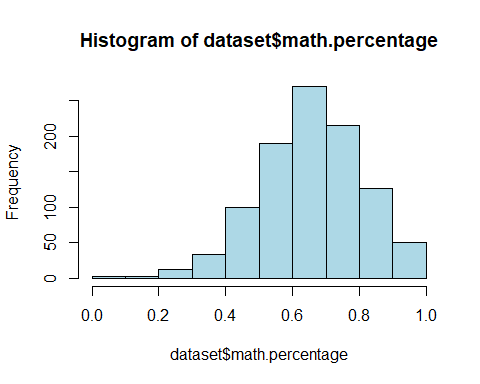
\includegraphics{ass1_files/figure-latex/unnamed-chunk-2-1.pdf}

\begin{Shaded}
\begin{Highlighting}[]
\FunctionTok{mean}\NormalTok{(dataset}\SpecialCharTok{$}\NormalTok{math.percentage)}
\end{Highlighting}
\end{Shaded}

\begin{verbatim}
## [1] 0.66089
\end{verbatim}

\begin{Shaded}
\begin{Highlighting}[]
\FunctionTok{median}\NormalTok{(dataset}\SpecialCharTok{$}\NormalTok{math.percentage)}
\end{Highlighting}
\end{Shaded}

\begin{verbatim}
## [1] 0.66
\end{verbatim}

\begin{Shaded}
\begin{Highlighting}[]
\FunctionTok{boxplot}\NormalTok{(dataset}\SpecialCharTok{$}\NormalTok{writing.score.percentage,}\AttributeTok{col =} \StringTok{\textquotesingle{}dark green\textquotesingle{}}\NormalTok{)}
\end{Highlighting}
\end{Shaded}

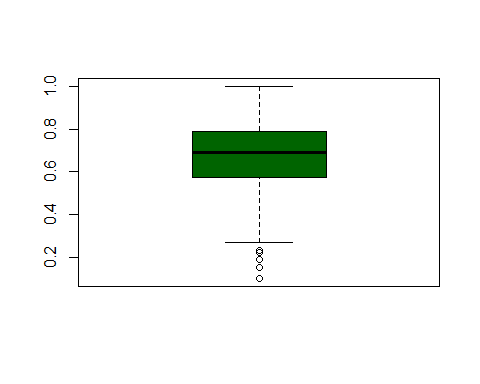
\includegraphics{ass1_files/figure-latex/unnamed-chunk-3-1.pdf}

\begin{Shaded}
\begin{Highlighting}[]
\DocumentationTok{\#\#\#Categorical Variables}
\FunctionTok{class}\NormalTok{(dataset}\SpecialCharTok{$}\NormalTok{sex)}
\end{Highlighting}
\end{Shaded}

\begin{verbatim}
## [1] "character"
\end{verbatim}

\begin{Shaded}
\begin{Highlighting}[]
\FunctionTok{table}\NormalTok{(dataset}\SpecialCharTok{$}\NormalTok{sex)}
\end{Highlighting}
\end{Shaded}

\begin{verbatim}
## 
##   F   M 
## 518 482
\end{verbatim}

\begin{Shaded}
\begin{Highlighting}[]
\NormalTok{mypct}\OtherTok{=}\FunctionTok{round}\NormalTok{((}\FunctionTok{table}\NormalTok{(dataset}\SpecialCharTok{$}\NormalTok{sex))}\SpecialCharTok{/}\NormalTok{(}\FunctionTok{sum}\NormalTok{(}\FunctionTok{table}\NormalTok{(dataset}\SpecialCharTok{$}\NormalTok{sex)))}\SpecialCharTok{*}\DecValTok{100}\NormalTok{)}
\NormalTok{lbls}\OtherTok{=}\FunctionTok{paste}\NormalTok{(}\FunctionTok{names}\NormalTok{(}\FunctionTok{table}\NormalTok{(dataset}\SpecialCharTok{$}\NormalTok{sex)),mypct,}\StringTok{"\%"}\NormalTok{)}
\FunctionTok{pie}\NormalTok{(}\FunctionTok{table}\NormalTok{(dataset}\SpecialCharTok{$}\NormalTok{sex),lbls,}\AttributeTok{main =} \StringTok{"Gender Percentage"}\NormalTok{)}
\end{Highlighting}
\end{Shaded}

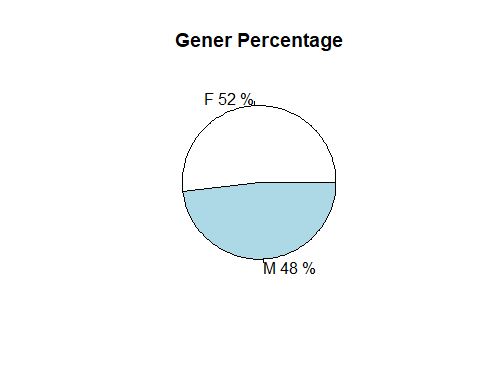
\includegraphics{ass1_files/figure-latex/unnamed-chunk-4-1.pdf}

\begin{Shaded}
\begin{Highlighting}[]
\DocumentationTok{\#\#\#variable transformation}

\DocumentationTok{\#\# adding new colmn for the GPA }
\FunctionTok{library}\NormalTok{(tidyverse)}
\end{Highlighting}
\end{Shaded}

\begin{verbatim}
## -- Attaching packages --------------------------------------- tidyverse 1.3.1 --
\end{verbatim}

\begin{verbatim}
## v ggplot2 3.3.5     v purrr   0.3.4
## v tibble  3.1.4     v dplyr   1.0.7
## v tidyr   1.1.3     v stringr 1.4.0
## v readr   2.0.1     v forcats 0.5.1
\end{verbatim}

\begin{verbatim}
## -- Conflicts ------------------------------------------ tidyverse_conflicts() --
## x dplyr::filter() masks stats::filter()
## x dplyr::lag()    masks stats::lag()
\end{verbatim}

\begin{Shaded}
\begin{Highlighting}[]
\NormalTok{dataset\_mutate }\OtherTok{\textless{}{-}}\NormalTok{ dataset }\SpecialCharTok{\%\textgreater{}\%} \FunctionTok{mutate}\NormalTok{(}\AttributeTok{GPA =}\NormalTok{ (dataset}\SpecialCharTok{$}\NormalTok{math.percentage }\SpecialCharTok{+}\NormalTok{ dataset}\SpecialCharTok{$}\NormalTok{reading.score.percentage }\SpecialCharTok{+}\NormalTok{ dataset}\SpecialCharTok{$}\NormalTok{writing.score.percentage)}\SpecialCharTok{/}\DecValTok{3}\NormalTok{)}
\FunctionTok{View}\NormalTok{(dataset\_mutate)}
\end{Highlighting}
\end{Shaded}

\begin{Shaded}
\begin{Highlighting}[]
\DocumentationTok{\#\#\# Plot }
\FunctionTok{plot}\NormalTok{(dataset}\SpecialCharTok{$}\NormalTok{writing.score.percentage,dataset}\SpecialCharTok{$}\NormalTok{reading.score.percentage,}\AttributeTok{col=}\StringTok{\textquotesingle{}black\textquotesingle{}}\NormalTok{)}
\end{Highlighting}
\end{Shaded}

\includegraphics{ass1_files/figure-latex/unnamed-chunk-6-1.pdf}

\begin{Shaded}
\begin{Highlighting}[]
\FunctionTok{plot}\NormalTok{(dataset}\SpecialCharTok{$}\NormalTok{math.percentage,dataset}\SpecialCharTok{$}\NormalTok{GPA,}\AttributeTok{col=}\StringTok{\textquotesingle{}black\textquotesingle{}}\NormalTok{)}
\end{Highlighting}
\end{Shaded}

\includegraphics{ass1_files/figure-latex/unnamed-chunk-7-1.pdf}

\hypertarget{source-of-the-data-set-httpswww.kaggle.comspscientiststudents-performance-in-exams}{%
\subsubsection{\texorpdfstring{SOURCE OF THE DATA SET
\url{https://www.kaggle.com/spscientist/students-performance-in-exams}}{SOURCE OF THE DATA SET https://www.kaggle.com/spscientist/students-performance-in-exams}}\label{source-of-the-data-set-httpswww.kaggle.comspscientiststudents-performance-in-exams}}

\end{document}
